% Options for packages loaded elsewhere
\PassOptionsToPackage{unicode}{hyperref}
\PassOptionsToPackage{hyphens}{url}
%
\documentclass[
]{ltjarticle}
\usepackage{graphicx}
\usepackage{svg}
\usepackage{grffile}
\usepackage{lmodern}
\usepackage{amssymb, amsmath}
\usepackage{ifxetex, ifluatex}
\usepackage{svg, graphicx, enumerate, amsmath, amsfonts, amssymb, wrapfig, here, float, url, multirow, subfigure, titlesec, siunitx, bm}
\ifnum 0\ifxetex 1\fi\ifluatex 1\fi=0 % if pdftex
  \usepackage[T1]{fontenc}
  \usepackage[utf8]{inputenc}
  \usepackage{textcomp} % provide euro and other symbols
\else % if luatex or xetex
  \usepackage{unicode-math}
  \defaultfontfeatures{Scale=MatchLowercase}
  \defaultfontfeatures[\rmfamily]{Ligatures=TeX, Scale=1}
\fi
% Use upquote if available, for straight quotes in verbatim environments
\IfFileExists{upquote. sty}{\usepackage{upquote}}{}
\IfFileExists{microtype. sty}{% use microtype if available
  \usepackage[]{microtype}
  \UseMicrotypeSet[protrusion]{basicmath} % disable protrusion for tt fonts
}{}
\makeatletter
\usepackage{svg}
\@ifundefined{KOMAClassName}{% if non-KOMA class
  \IfFileExists{parskip. sty}{%
    \usepackage{parskip}
  }{% else
    \setlength{\parindent}{0pt}
    \setlength{\parskip}{6pt plus 2pt minus 1pt}}
}{% if KOMA class
  \KOMAoptions{parskip=half}}
\makeatother
\usepackage{xcolor}
\IfFileExists{xurl. sty}{\usepackage{xurl}}{} % add URL line breaks if available
\IfFileExists{bookmark. sty}{\usepackage{bookmark}}{\usepackage{hyperref}}
\hypersetup{
  hidelinks, 
  pdfcreator={LaTeX via pandoc}}
\urlstyle{same} % disable monospaced font for URLs
\usepackage[margin=1in]{geometry}
\usepackage{graphicx, grffile}
\usepackage{listings}


\makeatletter
\def\maxwidth{\ifdim\Gin@nat@width>\linewidth\linewidth\else\Gin@nat@width\fi}
\def\maxheight{\ifdim\Gin@nat@height>\textheight\textheight\else\Gin@nat@height\fi}
\makeatother
% Scale images if necessary, so that they will not overflow the page
% margins by default, and it is still possible to overwrite the defaults
% using explicit options in \includegraphics[width, height, ... ]{}
\setkeys{Gin}{width=\maxwidth, height=\maxheight, keepaspectratio}
% Set default figure placement to htbp
\makeatletter
\def\fps@figure{htbp}
\makeatother
\setlength{\emergencystretch}{3em} % prevent overfull lines
\providecommand{\tightlist}{%
  \setlength{\itemsep}{0pt}\setlength{\parskip}{0pt}}
\setcounter{secnumdepth}{5}
\usepackage{listings}
\usepackage{xcolor}
 
\lstset{
    basicstyle=\ttfamily, 
    keywordstyle=\color[RGB]{33, 74, 135}\bfseries, 
    stringstyle=\color[RGB]{79, 153, 5}, 
    commentstyle=\color[RGB]{143, 89, 2}\itshape, 
    numberstyle=\footnotesize, 
    numbers=left, 
    stepnumber=1, 
    numbersep=15pt, 
    backgroundcolor=\color[RGB]{251, 251, 251}, 
    frame=single, 
    frameround=ffff, 
    framesep=5pt, 
    rulecolor=\color[RGB]{148, 150, 152}, 
    breaklines=true, 
    breakautoindent=true, 
    breakatwhitespace=true, 
    breakindent=25pt, 
    showspaces=false, 
    showstringspaces=false, 
    showtabs=false, 
    tabsize=2, 
    captionpos=b, 
    linewidth=\textwidth, 
}
\date{}
\usepackage{color}
\usepackage{listings, jlisting}

\lstset{
language={C}, 
backgroundcolor={\color[gray]{. 85}}, 
basicstyle={\small}, 
identifierstyle={\small}, 
commentstyle={\small\ttfamily \color[rgb]{0, 0. 5, 0}}, 
keywordstyle={\small\bfseries \color[rgb]{1, 0, 0}}, 
ndkeywordstyle={\small}, 
stringstyle={\small\ttfamily \color[rgb]{0, 0, 1}}, 
frame={tb}, 
breaklines=true, 
columns=[l]{fullflexible}, 
numbers=left, 
xrightmargin=0zw, 
xleftmargin=3zw, 
numberstyle={\scriptsize}, 
stepnumber=1, 
numbersep=1zw, 
morecomment=[l]{//}
}

\begin{document}
\section{機体のコンセプト}
\subsection{パワートレイン}
今回は 履帯駆動を採用した. 履帯駆動は通常の車輪よりも接地面積が大きいため, 地面が滑りやすくてもトルクが伝達できること, 左右どちらかの履帯を固定し, もう片方を駆動することで小回りがきく(信地旋回)などの利点がある. その反面, 駆動ロスが大きい, 騒音が発生する, \\ギアボックスとモーターは市販のキットを購入し, RA-130 モータを 58:1のギア比で使用し, 最高速度を重視した. 
\subsection{車体設計}
プラスチックの板を基礎にし, ギアボックスや履帯用のプーリー, ライントレース用センサーをネジ止めし, 電池ボックスは取り外しやすいようにマジックテープで取り付けた. 
\subsection{センサー部分}
市販のセンサーの配線を改造して使用した. 
\subsection{モータードライバー}
tc78h653ftg という 2 モーター出力できるモータドライバーを使用した. 
\section{自分の担当した箇所}
\subsection{ハードウェア}
\begin{itemize}
    \item   機体設計
    \begin{itemize}
        \item     コンセプトの考案
        \item     使用機材の選定(ユニバーサルプレート, ツインモータギヤボックス)
    \end{itemize}
    \item   基板設計
    \begin{itemize}
        \tightlist
        \item     Autodesk EAGLE を使用して基板を設計した. \\
            半田付けがしやすいように銅の幅をを大きくする, できるだけ一面で基板を作る などの工夫をした. 
        \item     電源設計\\
            FA-130 の定格電圧は 3V, モータドライバーの最大定格が 8Vだったので, 1.2V のニッケル水素畜電池を 6個直列に接続したものをモータドライバーに印加し, そこから三端子レギュレータで降圧した5V をマイコンなどに供給した. 
    \end{itemize}
    \item   基板製造\\
      高木君が組み立てた機体に基板を取り付けた. 
    \item   配線\\
      基板を取り付けた後に配線の長さを測り, 配線を取り付けた. 機体の一部に穴を開けて配線を通すようにすることで, ほかのものに配線がひっかからないようにした. 
    \end{itemize}
    \subsection{ソフトウェア}
    \begin{itemize}
    
    \item  API 作成\\
        もともとは複数人で開発する予定であったので, モーターや LED などが抽象化された API を作成した. 
    \item  PID 制御\\
        API 作成に時間がかかり, PID 制御は走行会までに実装できなかったが, 本来はライントレースを PID 制御で行う予定だった. 
\end{itemize}
\section{回路図と使用部品}
今回作成した基板の設計図を図1に表す. 
\begin{figure}[hbp]
    \centering
    \includegraphics[width=\linewidth]{report/fig1.png}
    \label{fig:fig1}
    \caption{基板の構成}
\end{figure}
    
DC ジャックが 2個あるのは, 電池一組で出力が足りなかった時のために用意した. 
プッシュスイッチは, スタートスイッチや, プログラムの切り替えなどに用いる予定だったが, 走行会までに実装できなかった. 
\newpage
\begin{table}[H]
    \label{tab1}
    \caption{今回使用した部品}
    \begin{center}
        \begin{tabular}{ccc}
    \hline
No. & 機器名& 型番など\\\hline
1&マイコン & PIC16F1778\\
2&モータードライバー & AE-C78H653FTG\\
3&ツインモータギヤボックス& タミヤ Item No:70097\\
4&トラック\&ホイールセット &タミヤ Item No:70100\\
5&ユニバーサルプレート&タミヤ Item No:70157\\
6&ライントレース用センーサ& AE-NJL5901AR-8CH\\\hline
    
\end{tabular}
\end{center}
\end{table}
\section{基板図}
今回作成した基板の設計図を図2に表す. 
\begin{figure}[H]
\centering
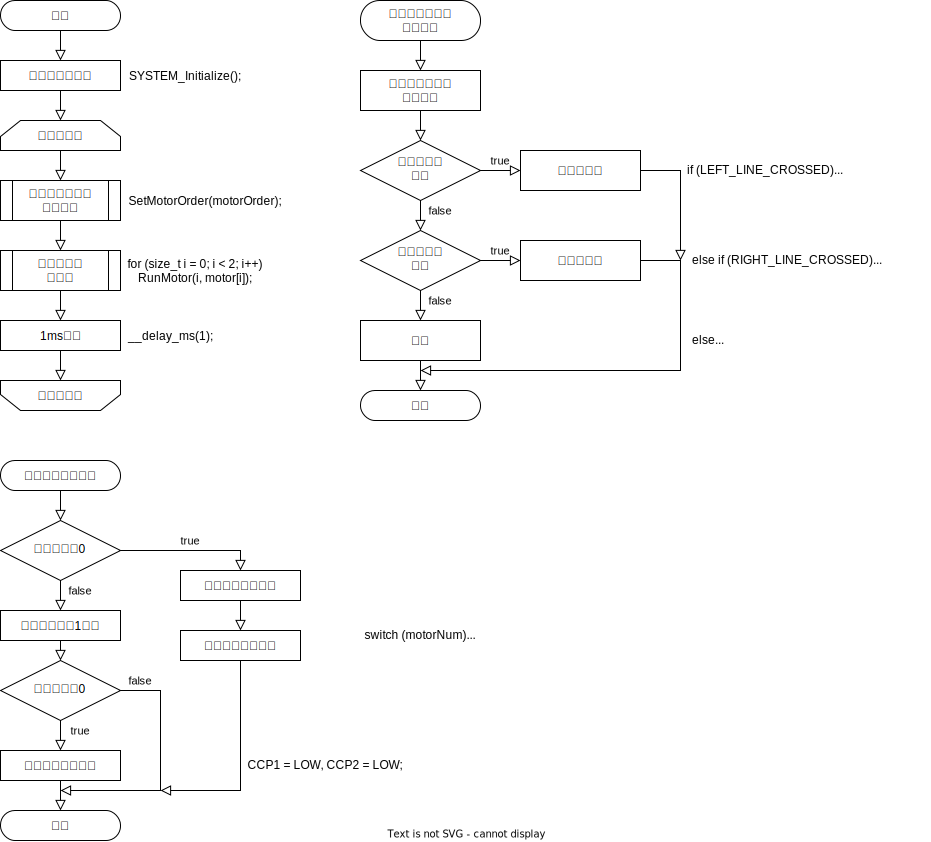
\includegraphics[width=\linewidth]{report/fig2.png}
\label{fig:fig2}
\caption{基板の構成}
\end{figure}
マイコンの電圧は 5V で, 発振器はPIC内部のものを使用した. 緑色や青色の部分は裏面の配線で, エッチング時に銅が残る範囲を表している. 白色の部分はマイコンなどの配置を表している. 赤い線の部分は裏面のみで配線できず, 表面に抵抗の足を使って接続した部分である. 
\section{フローチャート}
フローチャートを図3に表す. 
    割り込み処理でflagを変化させ, main関数でflagの値によって処理を分岐させる. 
\begin{figure}[H]
\centering
\includegraphics[width=\linewidth]{report/fig3.drawio.png}
\label{fig:fig3}
\caption{プログラムの構成}
\end{figure}
\section{走行会の結果}
9 月 27 日の走行会では, コースを完走することは出来なかった. PID 制御のプログラムが完成しなかったため, 急遽 ON/OFF 制御のプログラムに差し替えたが, ラインの検知が出来ず直進しかしなかった. 
\section{総括}
今回完走できなかった原因はプログラムに問題があったと思われる. モータードライバーへ PWM 信号を出力するときに, CCP機能ではなくタイマー割込みを用いて行った. 割込み周期が 4usと短すぎたため, 割込み処理の途中で割込みが発生していた. 改善点としては, PWM 信号は, CCP機能に任せてメインの処理に時間をさくこと, 割込み周期を下げ, 割込み処理中に割込みが入らないようにすること, 割込み処理の最初で割込みを禁止しておくことなどがあげられる. 
\section*{参考文献}
\begin{verbatim}
MPLAB® XC8 C Compiler User’s Guide: microchip 
http://ww1.microchip.com/downloads/en/devicedoc/50002053g.pdf
PICkit™ 3 Programmer/Debugger User’s Guide: microchip
 https://ww1.microchip.com/downloads/en/DeviceDoc/51795B.pdf
PIC16(L)F1777/8/9: microchip https://ww1.microchip.com/downloads/aemDocuments/documents/MCU08/
ProductDocuments/DataSheets/PIC16\%28L\%29F1777_8_9_Family_Data_Sheet_40001819D.pdf 
MPLAB® Code Configurator v3.xx User’s Guide: microchip
 http://ww1.microchip.com/downloads/en/devicedoc/40001829b.pdf
\end{verbatim}



\section*{付録: 今回作成したソースコードと解説}
1. main.c
\begin{verbatim}
#include "src/lineTracer.h"

void motorInit(void)
{
    setPort(&left, &LATB, IN2, IN1);
    setPort(&right, &LATB, IN4, IN3);
    setDirection(&left, true);
    setDirection(&right, true);
    MODE_LAT = LOW;
    LARGE_LAT = LOW;
    return;
}
void run(void)
{
    flag = !flag;
    return;
}
void main(void)
{
    SYSTEM_Initialize(), motorInit();
    setTargetSpeed(&left, leftSpeed);
    setTargetSpeed(&right, rightSpeed);
    TMR0_SetInterruptHandler(run);
    INTERRUPT_GlobalInterruptEnable();
    INTERRUPT_PeripheralInterruptEnable();
    while (true) {
        readLed(&led);
        autoPilot(&led, &leftSpeed, &rightSpeed);
        setTargetSpeed(&left, leftSpeed);
        setTargetSpeed(&right, rightSpeed);
        if (flag != flagOld) {
            flagOld = flag;
            runMotor(&left);
            runMotor(&right);
        }
    }
    return;
}
\end{verbatim}
2. src/lineTracer.h
\begin{verbatim}
#ifndef LINETRACER_H
#define LINETRACER_H

#include "../mcc_generated_files/mcc.h"
#include "LED.h"
#include "autoPilot.h"
#include "motor.h"

#define IN1 1 << 0
#define IN2 1 << 1
#define IN3 1 << 2
#define IN4 1 << 3

Motor left, right;
LED led;
uint8_t leftSpeed = 16, rightSpeed = 16;
bool flag = false, flagOld = false;
#endif
\end{verbatim}
\newpage
3. src/LED.h
\begin{verbatim}
#ifndef LED_H
#define LED_H

#include "../mcc_generated_files/mcc.h"
#include <stdbool.h>
#include <stdint.h>

typedef struct {
    bool _LED1;
    bool _LED2;
    bool _LED4;
    bool _LED5;
    bool _LED7;
    bool _LED8;
    adc_result_t _LED3A;
    adc_result_t _LED6A;
} LED;

void readLed(LED* self);

#endif
\end{verbatim}
\newpage
4. src/LED.c
\begin{verbatim}
#include "LED.h"

void readLed(LED* self)
{
    self->_LED1 = LED1_PORT;
    self->_LED2 = LED2_PORT;
    self->_LED4 = LED4_PORT;
    self->_LED5 = LED5_PORT;
    self->_LED7 = LED7_PORT;
    self->_LED8 = LED8_PORT;
    self->_LED3A = ADC_GetConversion(LED3A);
    self->_LED6A = ADC_GetConversion(LED6A);
    return;
}
\end{verbatim}
5. src/autoPilot.h
\begin{verbatim}
#ifndef AUTOPILOT_H
#define AUTOPILOT_H

#include "LED.h"
#include "lineTracer.h"
#include <stdbool.h>
#include <stdint.h>

#define Kp 0. 05
#define Ki 0. 0
#define Kd 0. 0
#define dt 0. 01

void autoPilot(LED* led, uint8_t* leftSpeed, uint8_t* rightSpeed);
void lineTrace(LED* led, uint8_t* leftSpeed, uint8_t* rightSpeed);

#endif
\end{verbatim}
\newpage
6. src/autoPilot.c
\begin{verbatim}
#include "autoPilot.h"

void autoPilot(LED* led, uint8_t* leftSpeed, uint8_t* rightSpeed)
{
    lineTrace(led, leftSpeed, rightSpeed);
    return;
}
void lineTrace(LED* led, uint8_t* leftSpeed, uint8_t* rightSpeed)
{
    int8_t error = (int8_t)led->_LED3A - (int8_t)led->_LED6A;
    double pid = Kp * error;
    *leftSpeed = (uint8_t)(*leftSpeed + 1 + pid);
    *rightSpeed = (uint8_t)(*rightSpeed + 1 - pid);
    asm("NOP");
    return;
}
\end{verbatim}
7. src/motor.h
\begin{verbatim}
#ifndef MOTOR_H
#define MOTOR_H

#include "../mcc_generated_files/mcc.h"
#include <stdbool.h>
#include <stdint.h>

#define BASETIME 32

typedef struct {
    uint8_t _speed;
    uint8_t _targetSpeed;
    int8_t _tempSpeed;
    int8_t _tempTime;
    uint8_t _addr1;
    uint8_t _addr2;
    int16_t _tempCount;
    bool _direction;
    volatile uint8_t* _port;
} Motor;

int getSpeed(const Motor* self);
int getDirection(const Motor* self);
void setSpeed(Motor* self, uint8_t value);
void setTargetSpeed(Motor* self, uint8_t value);
void setDirection(Motor* self, bool value);
void setPort(Motor* self, volatile uint8_t* port, uint8_t addr1, uint8_t addr2);
void runMotor(Motor* self);

#endif
\end{verbatim}
8. src/motor.c
\begin{verbatim}
#include "motor.h"

void setSpeed(Motor* self, uint8_t value)
{
    self->_speed = value;
    return;
}
void setTargetSpeed(Motor* self, uint8_t value)
{
    self->_targetSpeed = value;
    return;
}
void setDirection(Motor* self, bool value)
{
    self->_direction = value;
    return;
}
void setPort(Motor* self, volatile uint8_t* port, uint8_t addr1, uint8_t addr2)
{
    self->_port = port, self->_addr1 = addr1, self->_addr2 = addr2;
    return;
}
void runMotor(Motor* self)
{
    uint8_t tempVal = *self->_port;
    uint8_t temp = 0;
    if (self->_tempTime-- > 0) {
        if (self->_tempSpeed-- > 0)
            temp += self->_direction ? self->_addr1 : self->_addr2;
    } else {
        if (!((self->_tempCount++) % 1700)) {
            if (self->_targetSpeed > self->_speed)
                self->_speed += 1;
            else if (self->_targetSpeed < self->_speed)
                self->_speed -= 2;
        }
        self->_tempSpeed = ((self->_speed) > BASETIME) ? BASETIME : self->_speed;
        self->_tempTime = BASETIME;
    }
    *self->_port = (tempVal & ~(self->_addr1 | self->_addr2)) | 
                   (temp & (self->_addr1 | self->_addr2));
    return;
}

\end{verbatim}
\end{document}
